\begin{frame}
\frametitle{Breathing}
%\begin{columns}[c] % The "c" option specifies centered vertical alignment while the "t" option is used for top vertical alignment

%\column{.3\textwidth} % Left column and width
%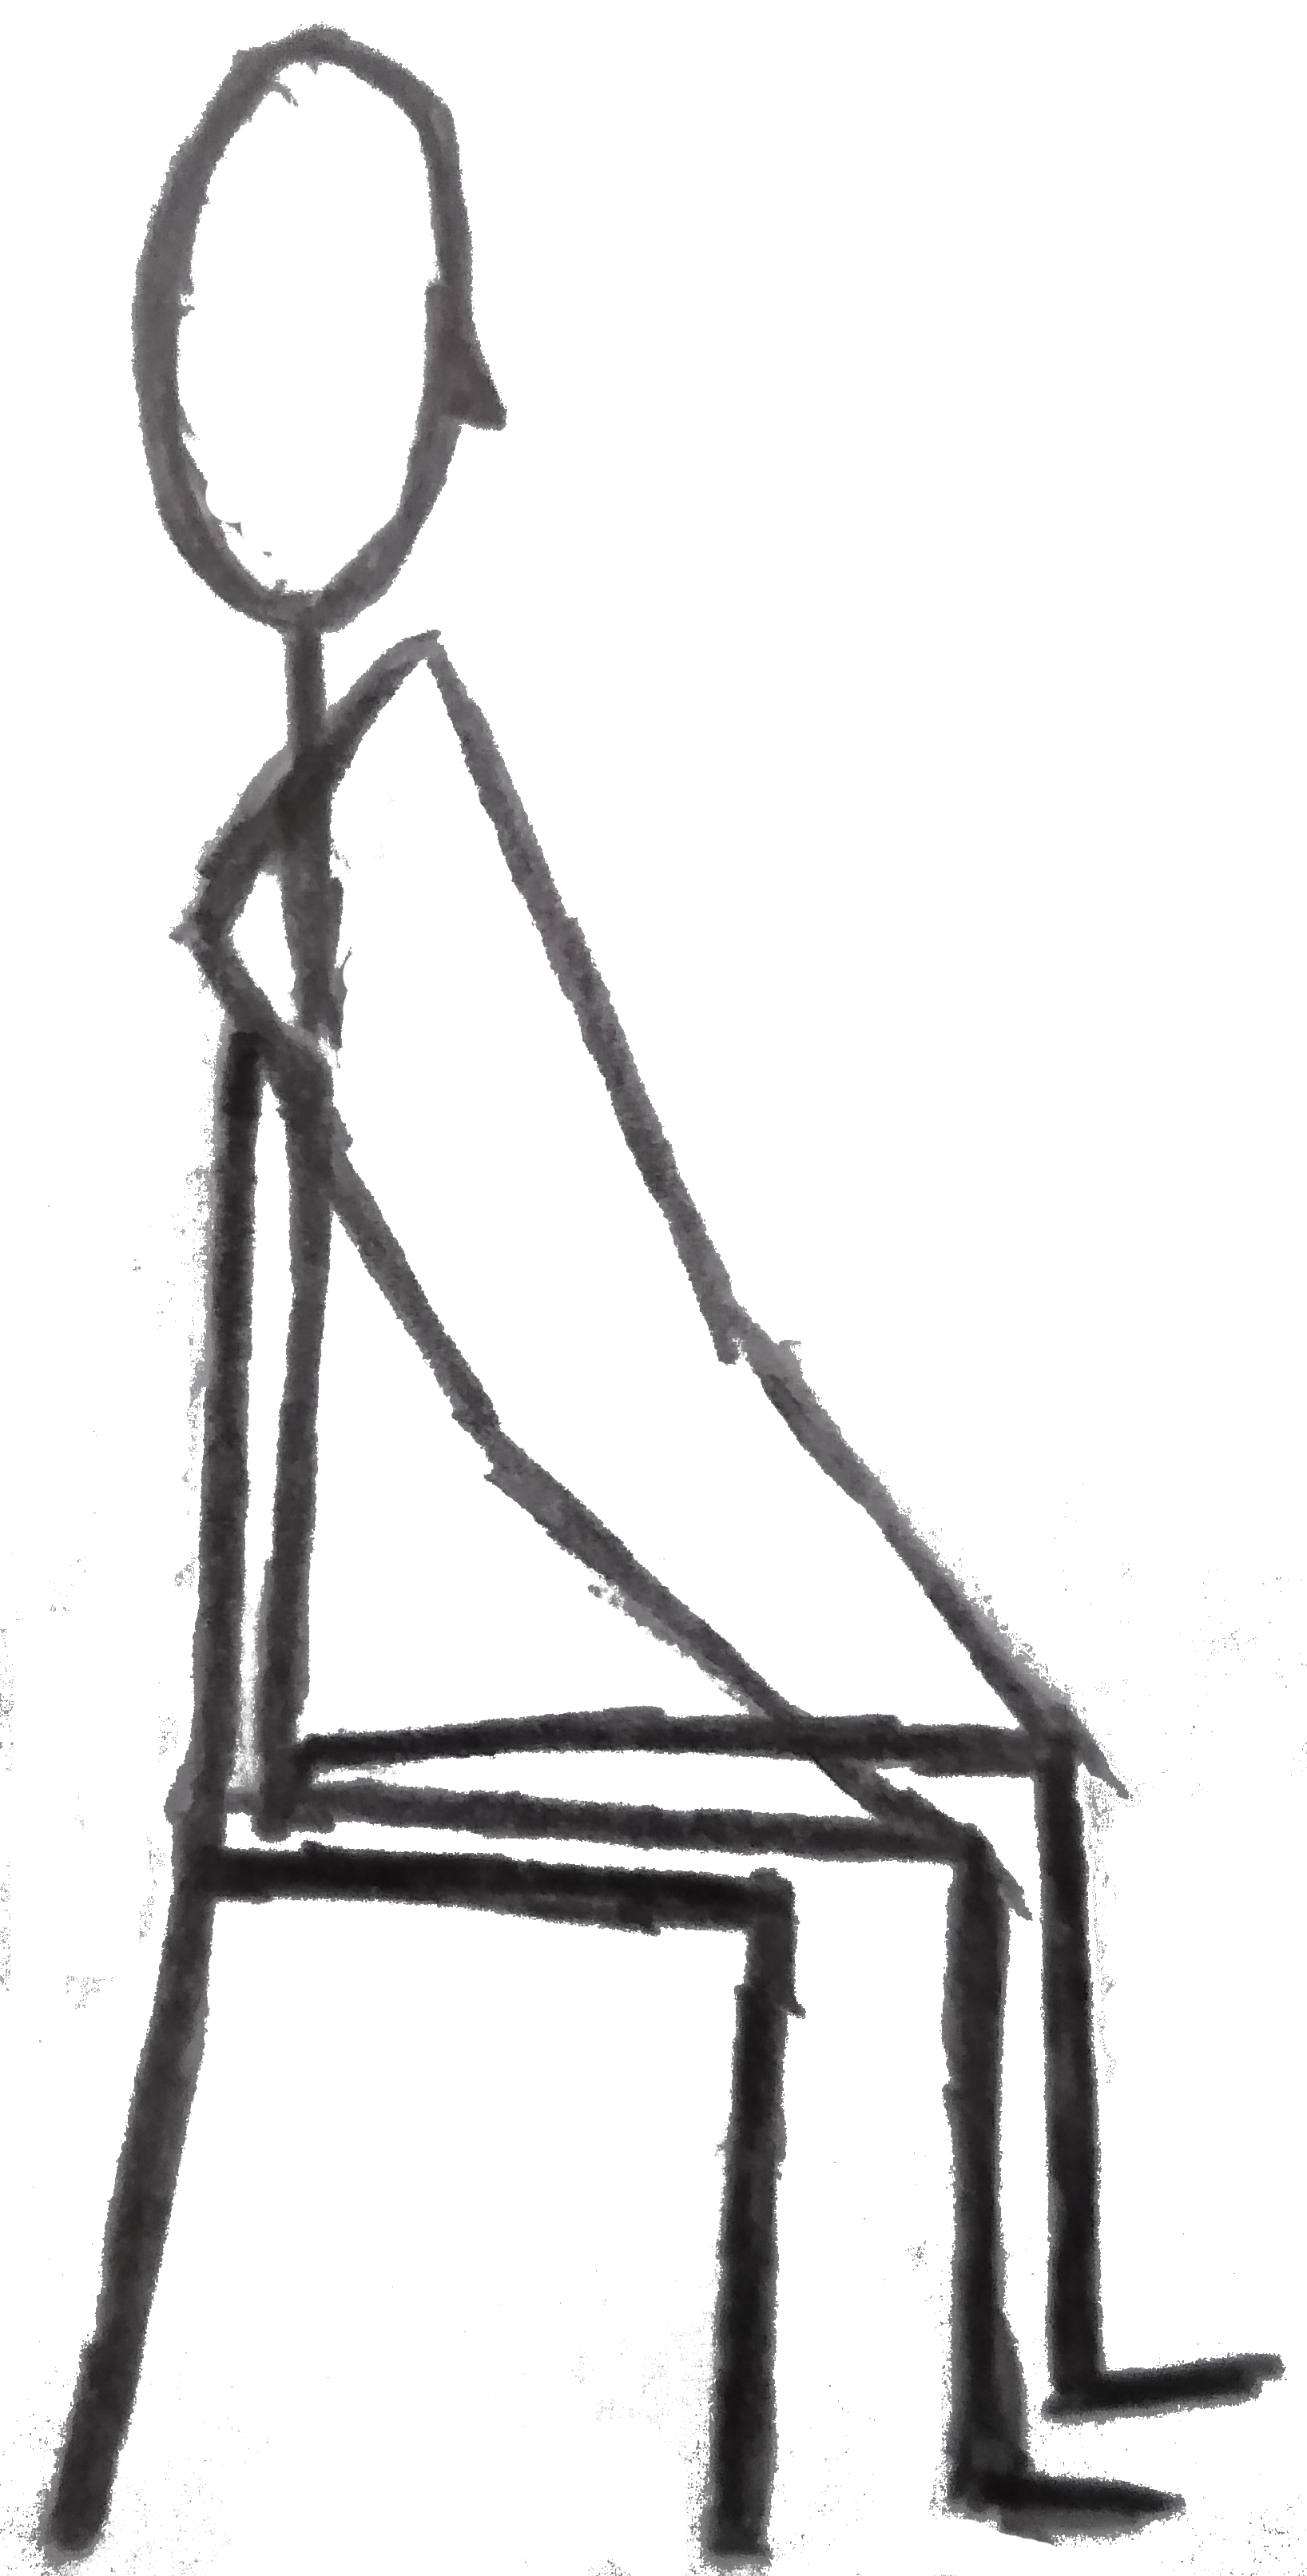
\includegraphics[width=\linewidth]{Sitting_chair_side.png}
%\column{.7\textwidth} % Right column and width
\begin{itemize}
\item[-] The \structure{breath} is of utmost importance for our \structure{health and well--being}.
\item[-] The nice things about is, that we can have an \structure{influence} on our \structure{breath}, therefore on \structure{our health and well--being}.
\item[-] When we are \structure{focussed, in joy, bored, in a hurry, physically active, angry, getting agitated or sad}, our breath goes along accordingly.
\item[-] Our \structure{breath adapts} to our state of being.
\item[-] \structure{Each unconscious function of our body} is in turn connected to the breath.
  \item[-] Breathing, depending on how we train it, \structure{builds up strenght} and \structure{equilibrates} missing or excessive things.
  \end{itemize}
% Write on
%\end{columns}
\end{frame}
%--------------------------------------------------------------------------------------------------------------

\begin{frame}
\frametitle{Perception of the Body}
%\begin{columns}[c] % The "c" option specifies centered vertical alignment while the "t" option is used for top vertical alignment

%\column{.3\textwidth} % Left column and width
%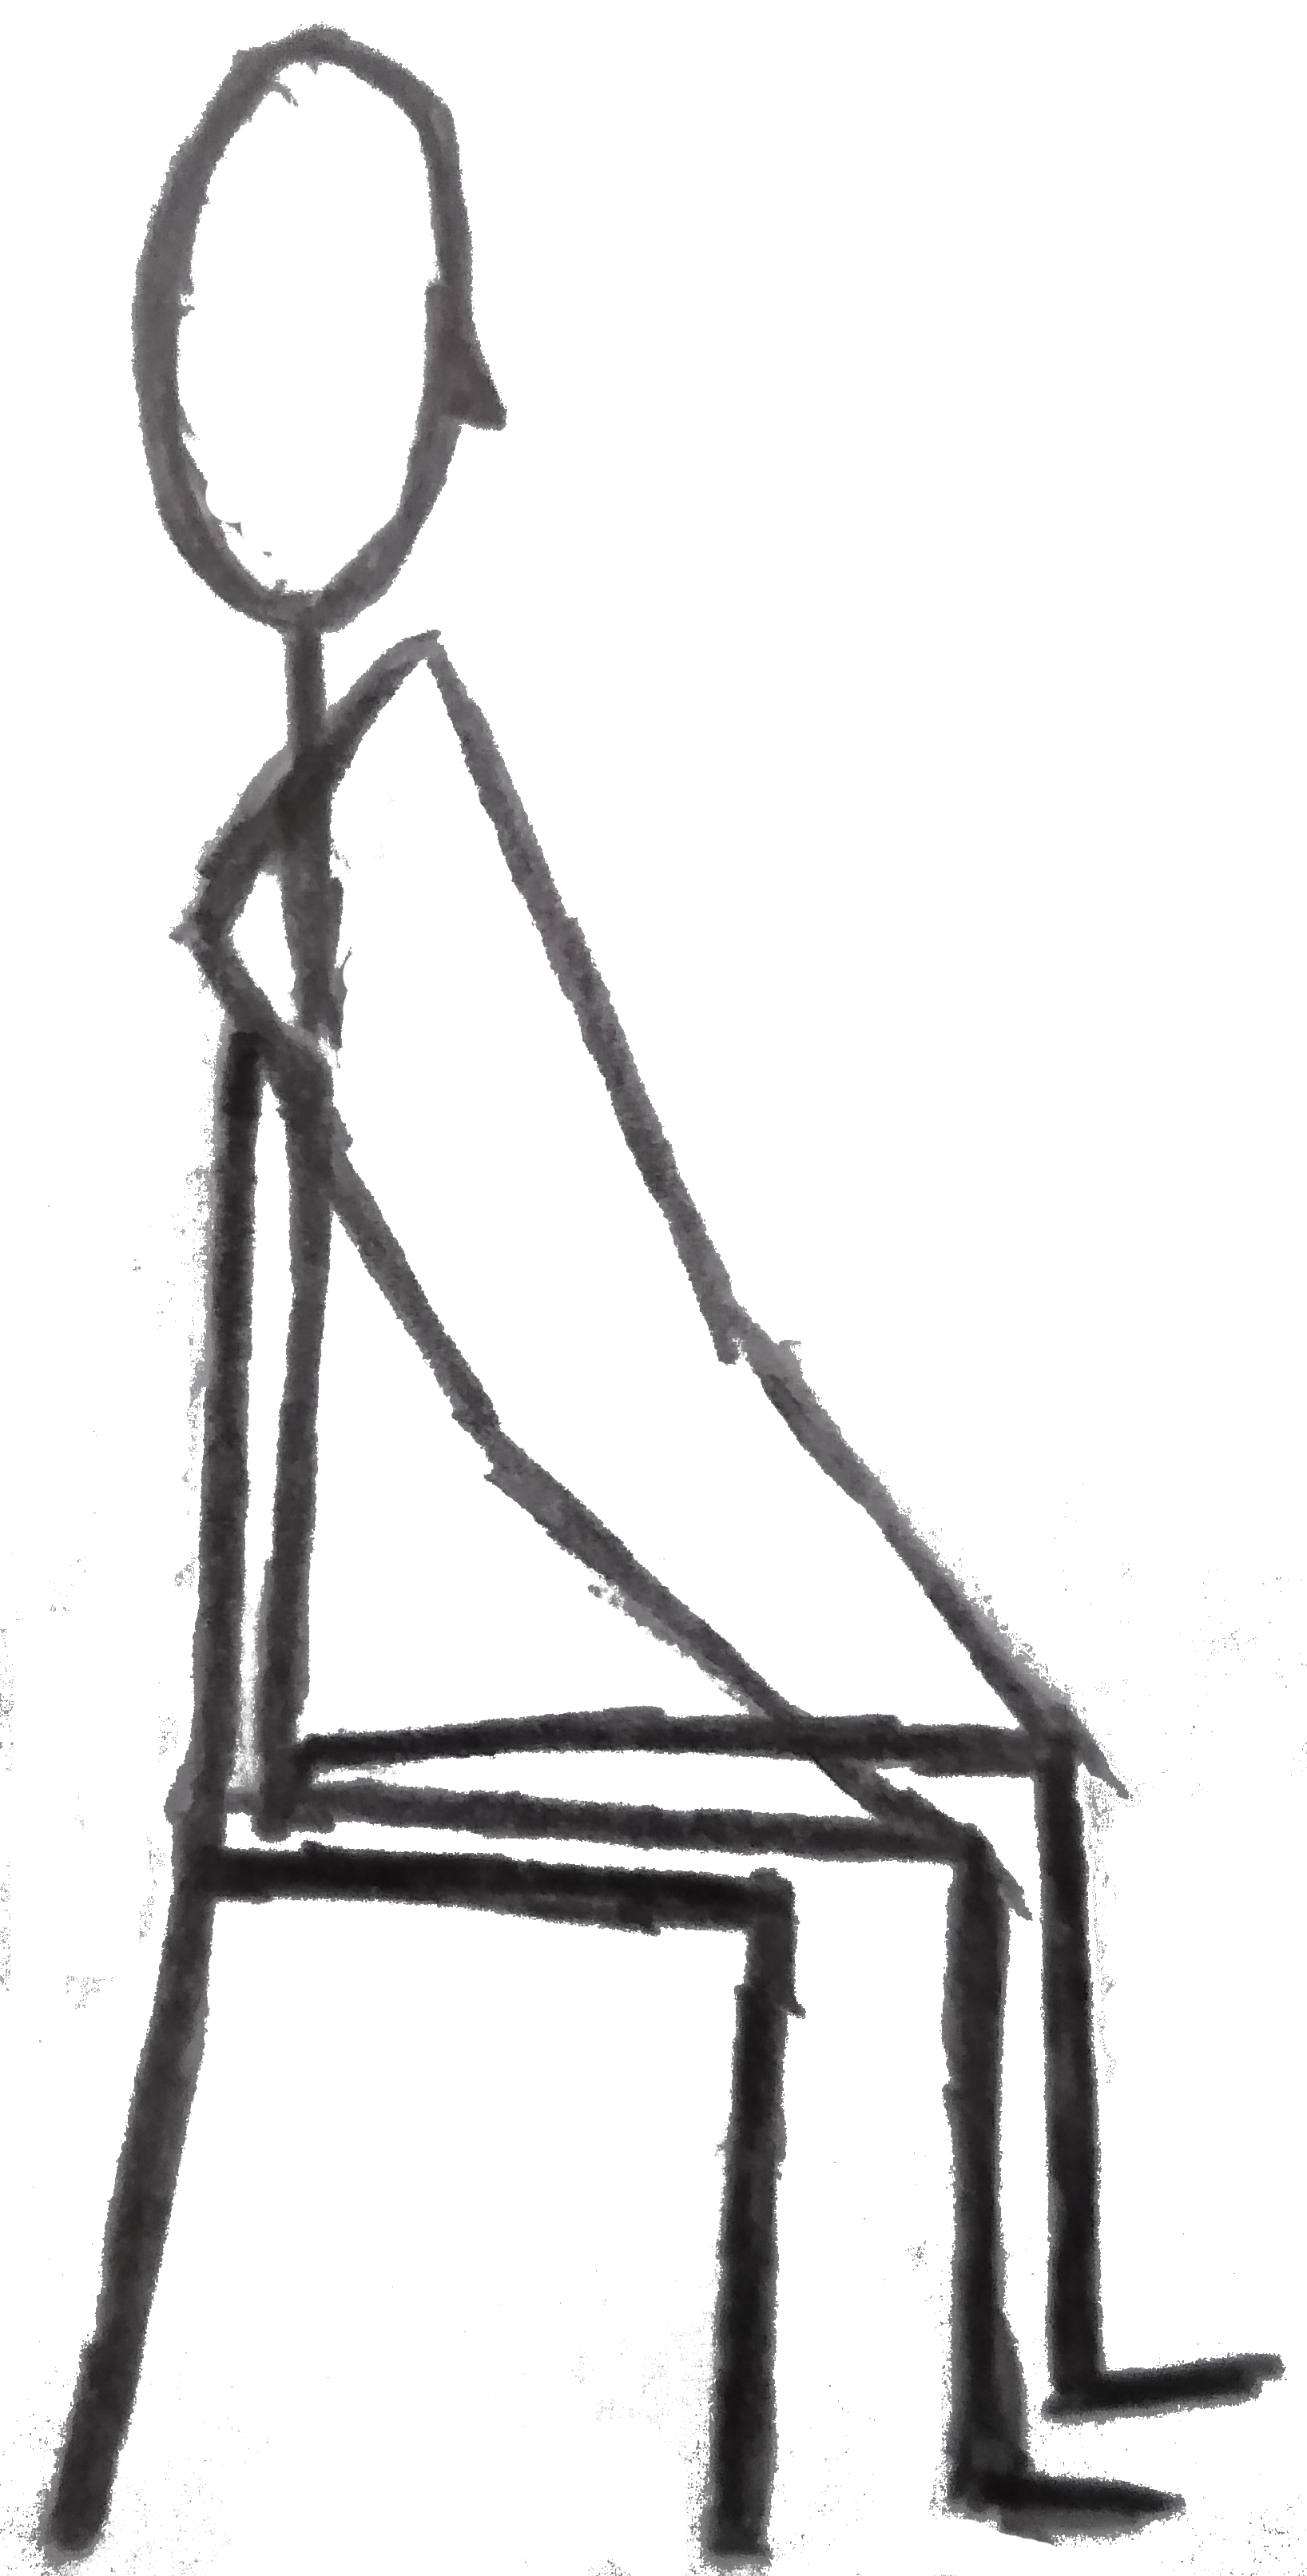
\includegraphics[width=\linewidth]{Sitting_chair_side.png}
%\column{.7\textwidth} % Right column and width
\begin{itemize}
\item[-] Conscious breathing also helps to better \structure{perceive your body} and therefore \structure{yourself}.
\item[-] Breathing is the \structure{instrument}, that you can lead through your body in a \structure{targeted and conscious way}.
\item[-] Your breath also leads you into a \structure{world of love}, as you are \structure{connected through your breath} with everybody and everything.
\item[-] In the framework of stress regulation, the breath is \structure{most immediately active tool}.
  \item[-] You can \structure{use it everywhere} and it's a natural tool --- and it also doesn't cost anything.
    \end{itemize}
% Write on
%\end{columns}
\end{frame}
%--------------------------------------------------------------------------------------------------------------

\begin{frame}
\frametitle{Basic principles}
%\begin{columns}[c] % The "c" option specifies centered vertical alignment while the "t" option is used for top vertical alignment

%\column{.3\textwidth} % Left column and width
%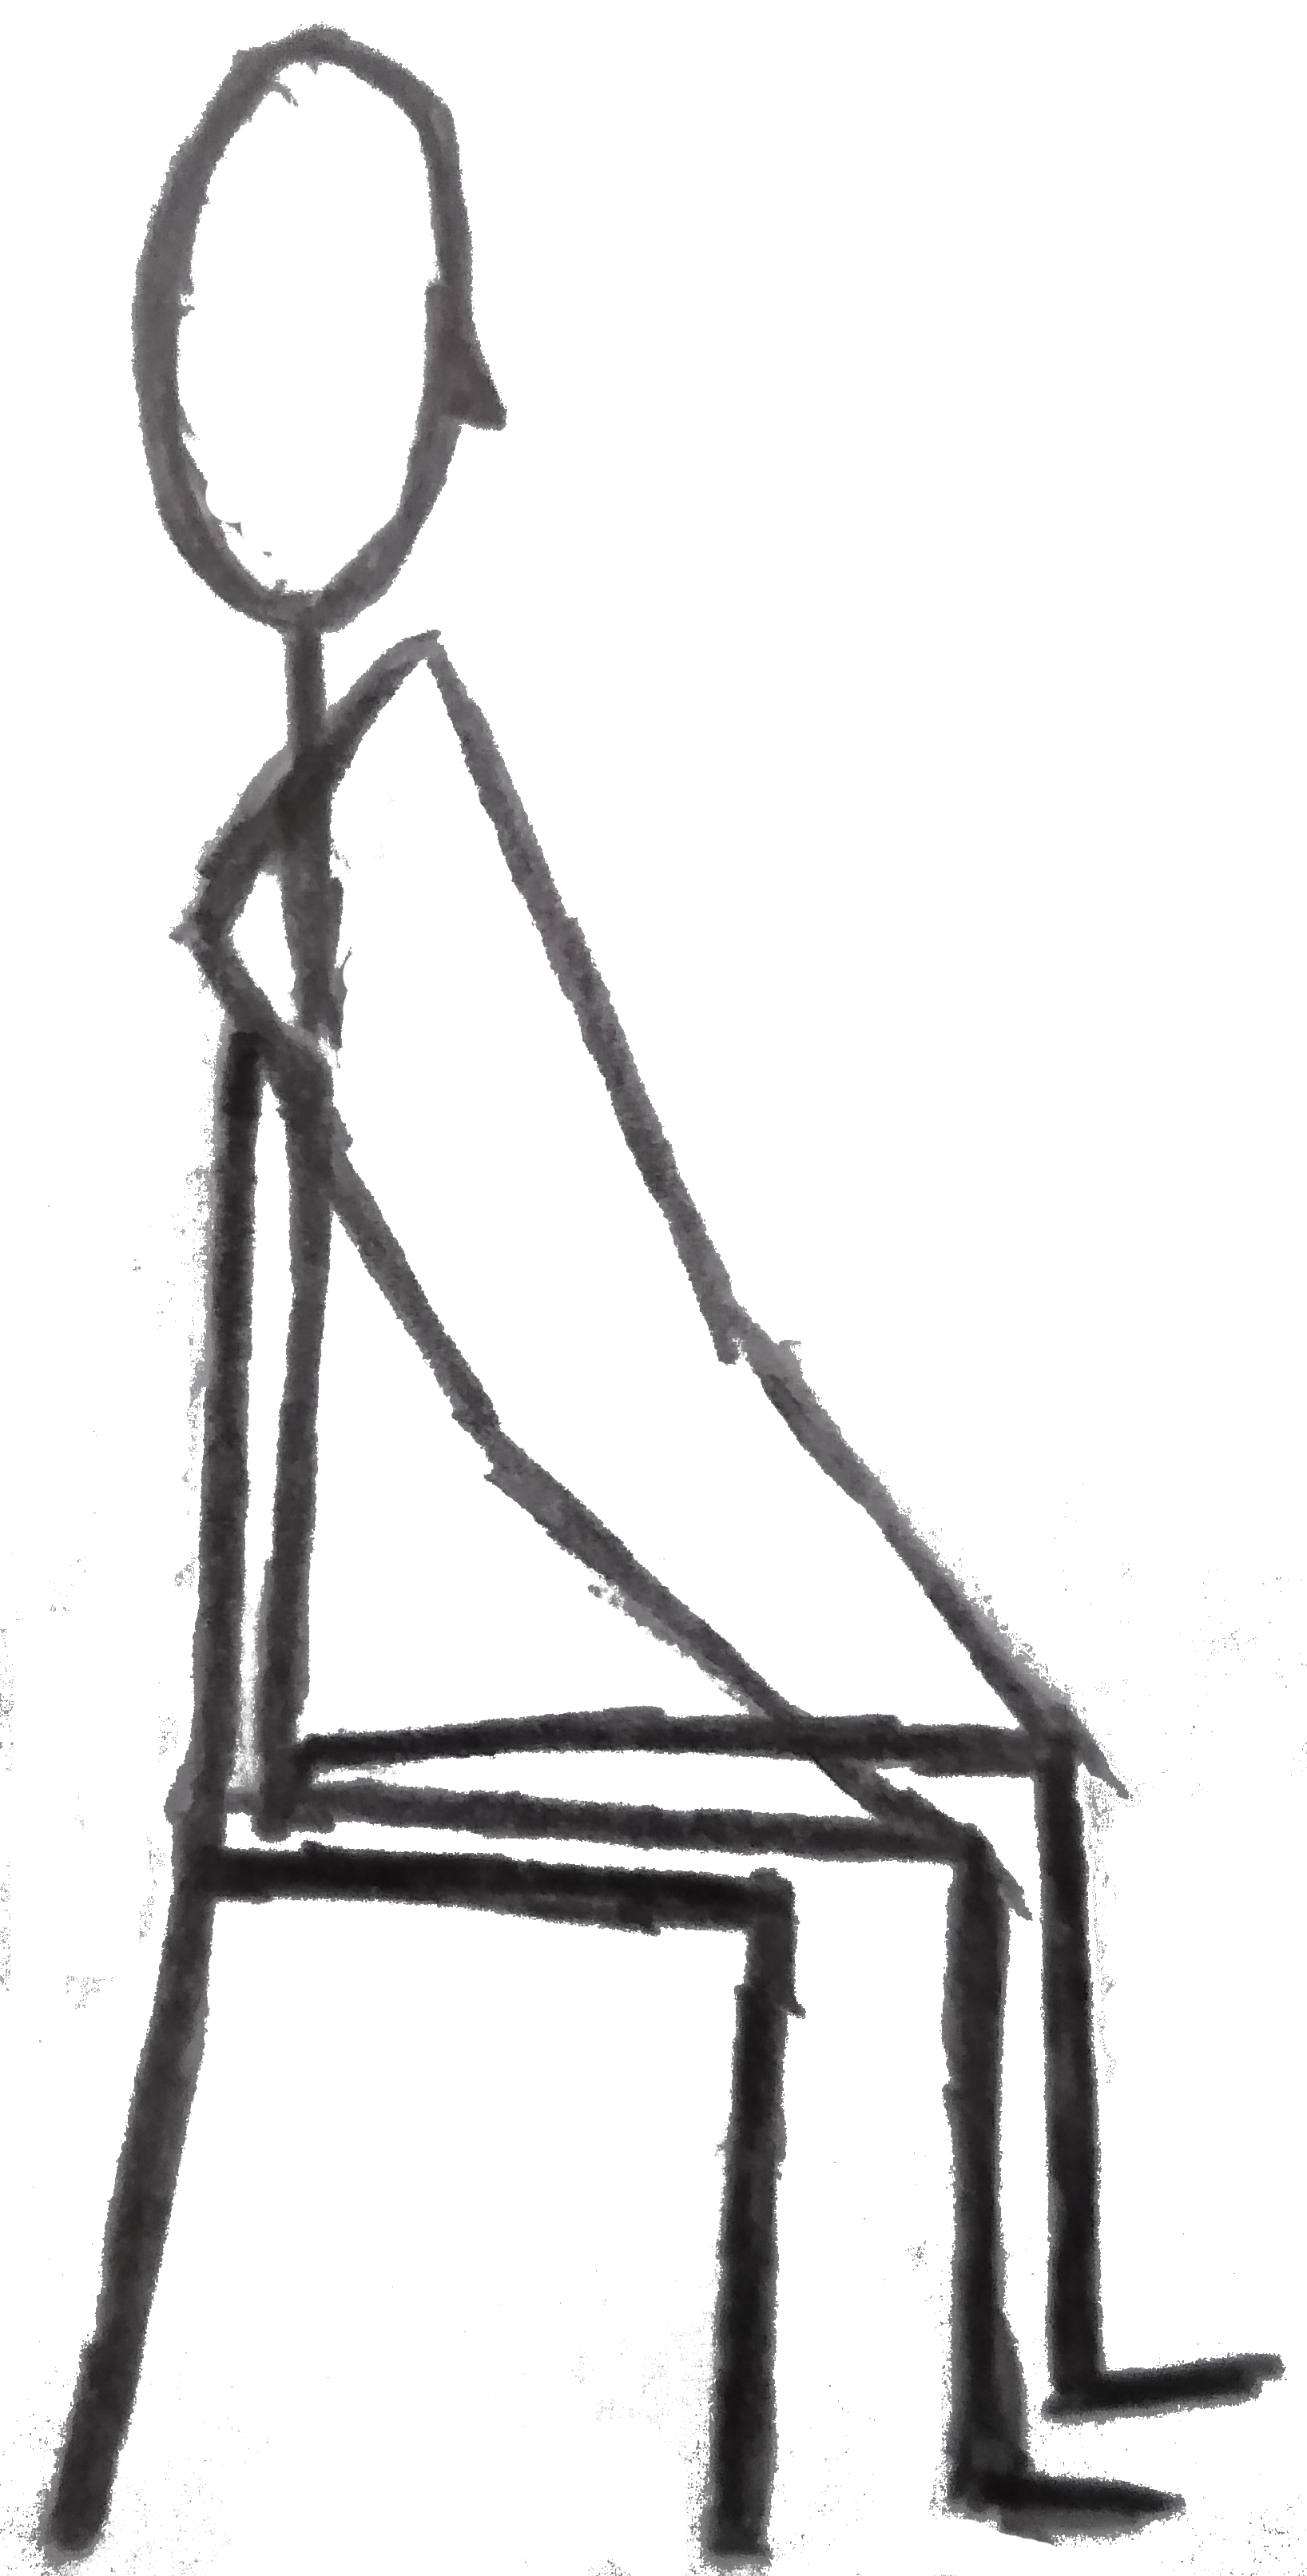
\includegraphics[width=\linewidth]{Sitting_chair_side.png}
%\column{.7\textwidth} % Right column and width
\begin{description}
\item[the inhale] \structure{builds up}, gives \structure{strength} and puts you \structure{back on your feet}.
\item[the exhale] \structure{relaxes}, calms down and \structure{loosens tension}.
  \end{description}

\begin{itemize}
\item[-] If you want to \structure{refresh}, build yourself up and get \structure{strength} --- \structure{prolong the inhale} and the \structure{pause} after the inhale.
\item[-] If you want to \structure{relax} and come to \structure{rest} --- \structure{slow down} and deepen the \structure{exhale}.
  \item[-] If you want to create an \structure{inner balance} --- pay attention to the inhale and exhale being \structure{regular}.
\end{itemize}

Don't force anything by doing that. \structure{Observe the rhythm} in a relaxed manner. When the \structure{thoughts are wandering} elsewhere, just bring them \structure{back to the breath}.
% Write on
%\end{columns}
\end{frame}
%--------------------------------------------------------------------------------------------------------------

